


%%%%%%%%%%%%%%%%%%%%%%%%%%%%%%%%%%%%%%%%%%%%%%%%%%%%%%%%%%%%%%%%%%%%%%%%%
%%%%%%%%%%%%%%%%%%%%%%%%%%%%%%%%%%%%%%%%%%%%%%%%%%%%%%%%%%%%%%%%%%%%%%%%%
%%%%%%%%%%%%%%%%%%%%%%%%%%%%%%%%%%%%%%%%%%%%%%%%%%%%%%%%%%%%%%%%%%%%%%%%%

\begin{frame}{The linear approximation.}

For $N=\SimNumObs$ data points, compute the OLS estimator from:

\vspace{1em}
\begin{tabularx}{\textwidth}{YYY}
%\begin{tabular}{ccc}
    Regressors  &   Residuals   &   Responses \\
    $x_n \sim \mathcal{N}(0, \sigma_x^2)$   &
    $\varepsilon_n \sim \mathcal{N}(0, \sigma_\varepsilon^2)$   &
    $y_n = \theta_0 x_n + \varepsilon_n$
\end{tabularx}
%

\SimApproxNormalGraph{}

\end{frame}


%%%%%%%%%%%%%%%%%%%%%%%%%%%%%%%%%%%%%%%%%%%%%%%%%%%%%%%%%%%%%%%%%%%%%%%%%
%%%%%%%%%%%%%%%%%%%%%%%%%%%%%%%%%%%%%%%%%%%%%%%%%%%%%%%%%%%%%%%%%%%%%%%%%
%%%%%%%%%%%%%%%%%%%%%%%%%%%%%%%%%%%%%%%%%%%%%%%%%%%%%%%%%%%%%%%%%%%%%%%%%


\begin{frame}{The linear approximation.}

\begin{minipage}[c]{0.25\textwidth}
    \hfill
\end{minipage}
\begin{minipage}[c]{0.49\textwidth}
\begin{centering}
%     \onslide<1-> {
%     Original weights: \par
%     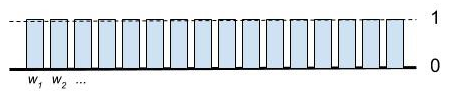
\includegraphics[width=0.68\textwidth]{static_figures/orig_weights}
%     }
%     \onslide<1-> {
%     \par Leave-one-out weights: \par
%     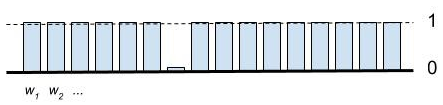
\includegraphics[width=0.68\textwidth]{static_figures/weights_loo}
%     }
%     \onslide<1-> {
%     \par Bootstrap weights: \par
%     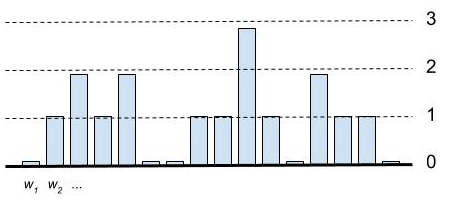
\includegraphics[width=0.68\textwidth]{static_figures/boot_weights}
%     }
% \end{minipage}
%\onslide<1->{
% \begin{minipage}{0.49\textwidth}
    % https://www.overleaf.com/learn/latex/TikZ_package
    % https://latexdraw.com/how-to-annotate-an-image-in-latex/
    % https://tex.stackexchange.com/questions/9559/drawing-on-an-image-with-tikz
\begin{tikzpicture}
    \node[anchor=south west,inner sep=0] (image) at (0,0) {
        %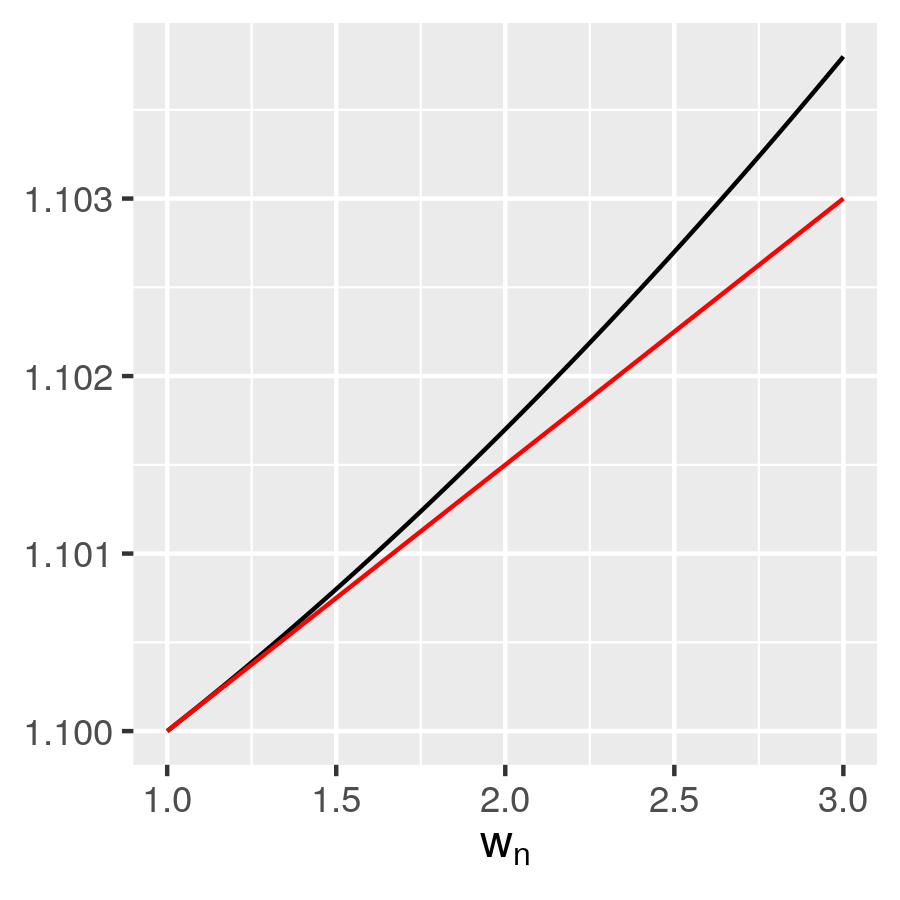
\includegraphics[width=0.98\textwidth]{static_figures/weight_slope}
        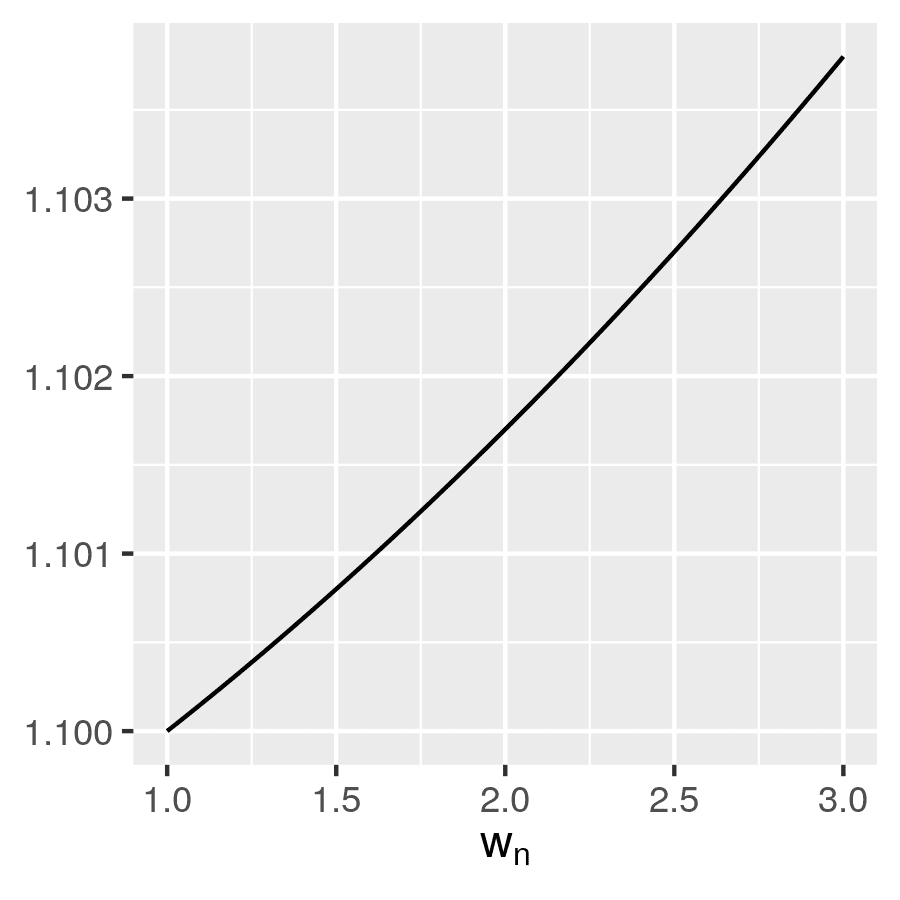
\includegraphics[width=0.98\textwidth]{static_figures/e_beta_w}
    };
    \begin{scope}[x={(image.south east)},y={(image.north west)}]
        \draw[blue, thick, <-] (0.2,0.23) -- ++(0.1,0.25)
                node[above,black,fill=white]
                {\small $\thetafun(\thetahat)$};
        \draw[blue, thick, <-] (0.8,0.8) -- ++(-0.1,0.1)
                node[left,black,fill=white]
                {\small $\thetafun(\thetahat(\w))$};
        \draw[red, thick, -] (0.18,0.18) -- ++(1.2 * 0.6, 1.2 * 0.48);
        \draw[blue, thick, <-] (0.8,0.65) -- ++(0.02,-0.1)
                node[below,black,fill=white]
                {\small Slope $ = \infl_n$};
    \end{scope}
\end{tikzpicture}
%}
\end{centering}
\end{minipage}

%
\begin{align*}
%
\thetafun(\thetahat(\w)) ={}&
\thetafun(\thetahat) + \sumn \infl_n (\w_n - 1) +
\textrm{Higher-order derivatives}
%
\end{align*}
%
\onslide<1->{
\vspace{-0.5em}
\textbf{Key idea: }
Controlling higher-order derivatives can control the error.
}

\end{frame}



%%%%%%%%%%%%%%%%%%%%%%%%%%%%%%%%%%%%%%%%%%%%%%%%%%%%%%%%%%%%%%%%%%%%%%%%%
%%%%%%%%%%%%%%%%%%%%%%%%%%%%%%%%%%%%%%%%%%%%%%%%%%%%%%%%%%%%%%%%%%%%%%%%%
%%%%%%%%%%%%%%%%%%%%%%%%%%%%%%%%%%%%%%%%%%%%%%%%%%%%%%%%%%%%%%%%%%%%%%%%%


\begin{frame}{The linear approximation.}
%
Let $W_\alpha$ be the set of weight vectors with no more than $\lfloor \alpha N
\rfloor$ zeros.

Let $H(\theta, \d_n) := \fracat{\partial G(\theta, \d_n)}{\partial
\theta^T}{\theta}$.

\begin{assu}[Smooth Objective]\assulabel{smooth}
Fix the dataset.
Assume there exists a compact $\thetadom \subseteq \mathbb{R}^D$
with $\thetahat(\w) \in \thetadom$ for all $\w \in W_\alpha$.
Assume that, for all $\theta \in \thetadom$:
%
\begin{itemize}
    \item $\meann H(\theta, \d_n)$ and $\meann G(\theta, \d_n)$ are bounded.
    \item $\meann H(\theta, \d_n)$ is uniformly non-singular and
    Lipschitz (in $\theta$).
    \item $\thetafun(\theta)$ has a Lipschitz first derivative.
\end{itemize}
%
\end{assu}

\begin{center}
\begin{tikzpicture}
    \draw[black, ->] (0,0) -- ++(0, 2.5);
    \draw[black, ->] (0,0) -- ++(0.5 * \textwidth, 0);
    \node[left] at (0, 2.3)
        {$\meann F(\theta, \d_n)$};
    \node[right] at (0.5 * \textwidth, 0) {$\theta$};
    \draw[fill=black, fill opacity=0.2, draw opacity=0]
        (0.1 * \textwidth, 0) rectangle ++(0.2 \textwidth, 2.5);
    \node[above] at (0.15 \textwidth, 0)
        {$\thetadom$};
    \node at (0.2 * \textwidth, 2.3) [circle,fill,inner sep=1pt]{};
    % \draw (0,0.9) .. controls
    %     (0.1 \textwidth, 2.0) and
    %     (0.2 \textwidth, 2.0) and
    %     (0.3 \textwidth, 0.8) and
    %     (0.4 \textwidth, 0.5) and
    %     .. (0.5 \textwidth, 1.2);
    \draw [black] plot [smooth, tension=0.6]
        coordinates {
            (0, 0.1)
            (0.1 * \textwidth, 1.9)
            (0.2 * \textwidth, 2.3)
            (0.3 * \textwidth, 1.9)
            % (0.3 * \textwidth, 1.6)
            (0.4 * \textwidth, 0.6)
            (0.5 * \textwidth, 0.8)
            };
\end{tikzpicture}
\end{center}

\end{frame}


%%%%%%%%%%%%%%%%%%%%%%%%%%%%%%%%%%%%%%%%%%%%%%%%%%%%%%%%%%%%%%%%%%%%%%%%%
%%%%%%%%%%%%%%%%%%%%%%%%%%%%%%%%%%%%%%%%%%%%%%%%%%%%%%%%%%%%%%%%%%%%%%%%%
%%%%%%%%%%%%%%%%%%%%%%%%%%%%%%%%%%%%%%%%%%%%%%%%%%%%%%%%%%%%%%%%%%%%%%%%%

\begin{frame}[t]{The linear approximation.}
%
\begin{theorem}\thmlabel{accurate}
%
Let \assuref{smooth} hold for a given dataset.
Then there exists a sufficiently small $\alpha$ such that
%
\begin{align*}
%
\sup_{\w \in W_\alpha} \abs{\thetafunlin(\w) - \thetafun(\thetahat(\w))}
    \le{}& C_1 \alpha \textrm{ and }
\sup_{\w \in W_\alpha} \abs{\thetafun(\thetahat(\w)) - \thetafun(\thetahat)}
    \le{} C_2 \sqrt{\alpha},
%
\end{align*}
%
where $C_1$ and $C_2$ are given by the quantities in the assumption.
%
\end{theorem}

\only<2>{
\vspace{1em}
Since $\alpha \ll \sqrt{\alpha}$ when $\alpha$ is small, \thmref{accurate}
states that the linear approximation's error is of smaller order than the actual
difference.
}

\only<3->{
\begin{proof}[Proof sketch.]
    % All derivatives can be given by the implicit function theorem.

    The second inequality follows from the smoothness of the objective.

    The first inequality follows from the smoothness of
    $d \thetahat(\w) / d\w$.
\end{proof}
}

\only<4>{
\begin{cor}
%
Under standard conditions, \assuref{smooth} holds for fixed constants with
probability approaching one for $N \rightarrow \infty$. Then \thmref{accurate}
applies with probability approaching one as $N \rightarrow \infty$.
%
\end{cor}
}

\end{frame}





%%%%%%%%%%%%%%%%%%%%%%%%%%%%%%%%%%%%%%%%%%%%%%%%%%%%%%%%%%%%%%%%%%%%%%%%%
%%%%%%%%%%%%%%%%%%%%%%%%%%%%%%%%%%%%%%%%%%%%%%%%%%%%%%%%%%%%%%%%%%%%%%%%%
%%%%%%%%%%%%%%%%%%%%%%%%%%%%%%%%%%%%%%%%%%%%%%%%%%%%%%%%%%%%%%%%%%%%%%%%%

\begin{frame}{Microcredit.}

{
\footnotesize
\MicrocreditProfitResultsTable{}
}

\end{frame}



\begin{frame}{Cash transfers.}

{
\footnotesize
\CashTransfersResultsTable{}
}

\end{frame}
